\documentclass[oneside,11pt,openright]{report}

\usepackage[latin1]{inputenc}
\usepackage[american]{babel}
\usepackage{a4}
\usepackage{latexsym}
\usepackage{rotating}
\usepackage{amsmath}
\usepackage{epsfig}
\usepackage[T1]{fontenc}
\usepackage{lmodern}
\usepackage{color}
\usepackage[table]{xcolor}
\usepackage{tabularx}
\usepackage{pdflscape}
\usepackage{datetime}
\usepackage{epstopdf}
\usepackage{soul}
\usepackage{graphicx}
\usepackage[font={small,it}]{caption}
\usepackage{subcaption}
\usepackage[authoryear]{natbib} % numbers or authoryear
\usepackage{amssymb}% http://ctan.org/pkg/amssymb
\usepackage{pifont}% http://ctan.org/pkg/pifont

% http://willbenton.com/wb-images/pifont.pdf
\newcommand{\cmark}{\ding{51}}%
\newcommand{\xmark}{\ding{55}}%


\renewcommand*\ttdefault{txtt}

\newcommand{\todo}[1]{{\color[rgb]{.5,0,0}\textbf{$\blacktriangleright$#1$\blacktriangleleft$}}}

% see http://imf.au.dk/system/latex/bog/

\begin{document}

%%%%%%%%%%%%%%%%%%%%%%%%%%%%%%%%%%%%%%%%%%%%%%%%%%%%%%%%%%%%%%%%%%%%%%%

% Used for table cells
\definecolor{TrueColor}{RGB}{209, 243, 209}
\definecolor{FalseColor}{RGB}{255, 204, 202}

\pagestyle{empty} 
\pagenumbering{roman} 
\vspace*{\fill}\noindent{\rule{\linewidth}{1mm}\\[4ex]
{\Huge\sf Flygtige interf\ae ses }\\[2ex]
{\huge\sf Tore Stubbe Lundgren, 20072415}\\[2ex]
{\huge\sf Stefan Andreas Bugge Loeschcke, 20073986}\\[2ex]
\noindent\rule{\linewidth}{1mm}\\[4ex]
\noindent{\Large\sf Master's Thesis, Computer Science\\[1ex] 
\monthname\ \the\year  \\[1ex] Advisor: Marianne Graves Petersen\\[15ex]}\\[\fill]}
\epsfig{file=logo.eps}\clearpage

%%%%%%%%%%%%%%%%%%%%%%%%%%%%%%%%%%%%%%%%%%%%%%%%%%%%%%%%%%%%%%%%%%%%%%%

\pagestyle{plain}
\chapter*{Abstract}
\addcontentsline{toc}{chapter}{Abstract}

\todo{in English\dots}

\chapter*{Resum\'e}
\addcontentsline{toc}{chapter}{Resum\'e}

\todo{in Danish\dots}

\chapter*{Acknowledgements}
\addcontentsline{toc}{chapter}{Acknowledgments}

\todo{\dots}

\vspace{2ex}
\begin{flushright}
  \emph{Tore Stubbe Lundgren and Stefan Andreas Bugge Loeschcke,}\\
  \emph{Aarhus, \today.}
\end{flushright}

\tableofcontents
\pagenumbering{arabic}
\setcounter{secnumdepth}{2}

\definecolor{HighLightColor}{RGB}{138,179,255}
\sethlcolor{HighLightColor}  % set highlighting color
%sethlcolor{}     %turn highlighting off -- I came back to turn the highlighting off once the changes were approved.

%%%%%%%%%%%%%%%%%%%%%%%%%%%%%%%%%%%%%%%%%%%%%%%%%%%%%%%%%%%%%%%%%%%%%%%

\chapter{Introduction}
\label{ch:intro}
%!TEX root = thesis.tex

\section{Motivation}
\label{ch:intro/motiv}
%!TEX root = ../thesis.tex
In this chapter we will attempt to bring together some of the ideas that has laid the ground and motivation for our thesis work.
Our process has not been on an entirely straight line, so at the same time we will try to draw lines between the different areas and disciplines that have shaped and influenced our process and ideas into the end result we present in this thesis.  

The original basis for this thesis was born from a fascination of objects that have the potential to combine the physical properties of solid objects with properties from world of computers and bits where objects moves, adapts and changes. 
In some sense bringing ``life'' to the objects and environments that surrounds us by letting them transform to our needs, both in function and form. 

The fascination of giving life to inanimate objects is not entirely new.
A famous example of this is the Vaucanson Duck, an automata created by the French inventor and artist Jacques Vaucanson in 1739 \citep{riskin2003defecating}.
It was later depicted by a nineteenth-century inventor, as seen in figure~\ref{vaucanson_duck} 
The mechanical duck, which supposedly contained over a thousand parts, could both flap its wings and appeared to have the ability to eat, digest, and defecate grains.

The animation of `things' still amazes today, both in the world of technology, with advancements in robotics, and in the world of crafts where ingenuity and craftsmanship can give rise to fascination.   
An example of the latter is Theo Jansen's that gives life to new species of animals with his amazing Strandbeests\footnote{http://www.strandbeest.com/}.  
Made mostly from yellow plastic tube and fabric sails, these skeletons traverses the beaches of the Netherlands, living off the wind, adapting to the turnings of the elements, see figure~\ref{strandbeest}.

\begin{figure}[h]
	\centering
	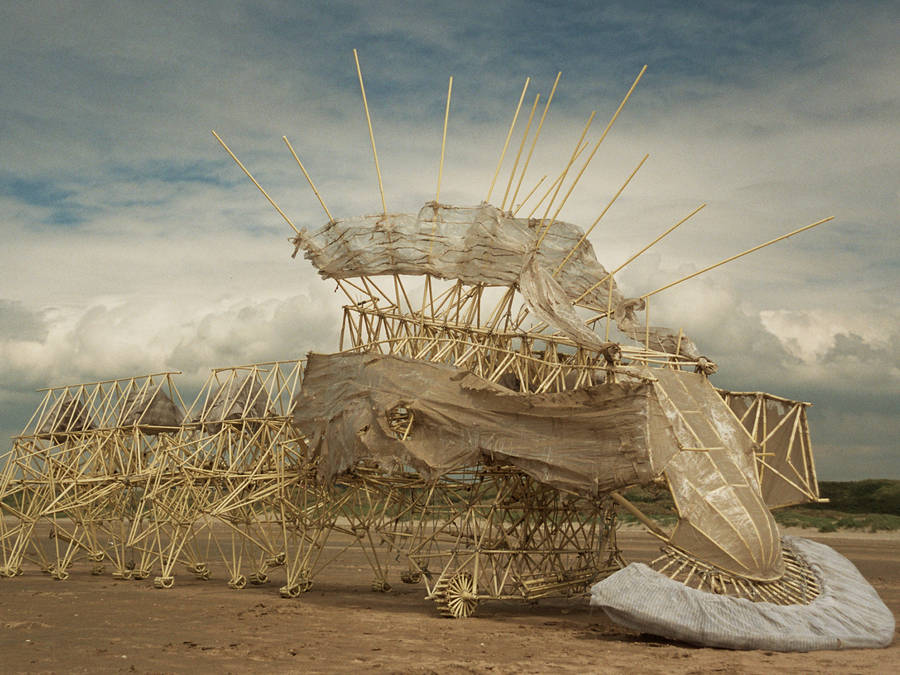
\includegraphics[width=0.9\linewidth]{figures/strandbeest}
	\captionof{figure}{One of Jansen's Strandbeests}
   	\label{strandbeest}
\end{figure}

\begin{figure}[h]
	\centering
	\begin{minipage}[b]{.8\textwidth}
		\centering
		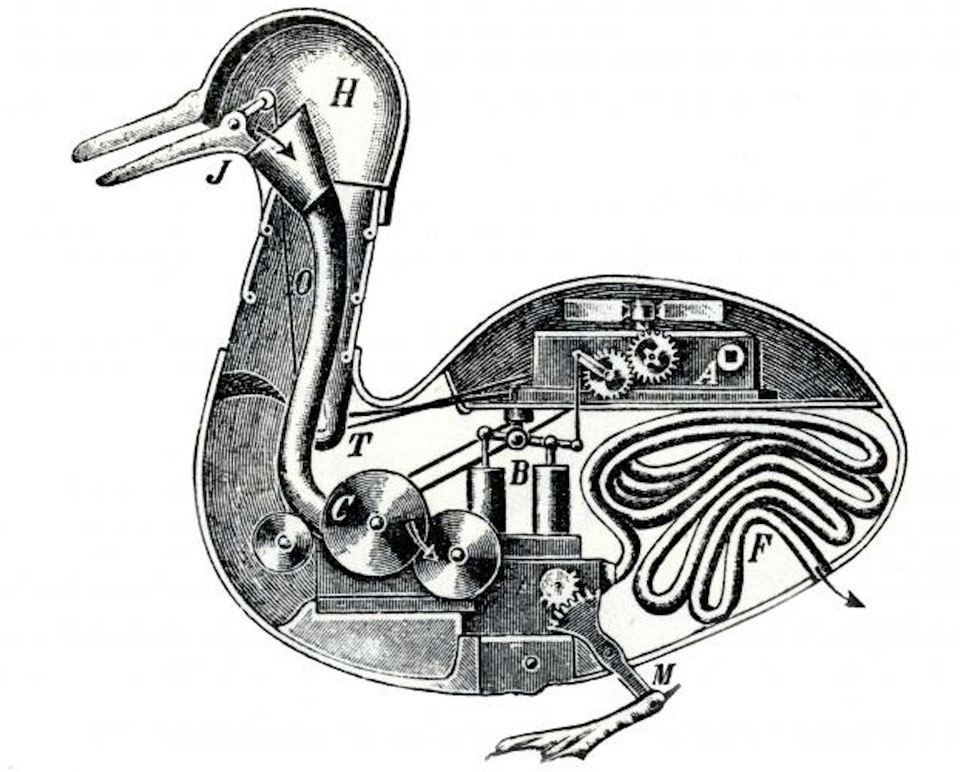
\includegraphics[width=.7\linewidth]{figures/vaucanson_duck}
		\captionof{figure}{A nineteenth-century inventor's imagined depiction of the inner workings of the Vaucanson Duck \citep{riskin2003defecating}}
		\label{vaucanson_duck}
	\end{minipage}
\end{figure}

These two examples, each impressive in their own right, points to the powerful expressiveness that actuation can give objects, as we have a tendency to relate things that move to living entities. 
\blank  
Looking back at traditional computing systems, before the era of Ubiquitous Computing \citep{weiser1991computer}, there has been a strong separation between the digital bits and the material world surrounding us.
The tangibility of digital information was then, for the most part, limited to keyboards and mice, icons and windows. 
And even though metaphors and graphical representations has helped us visualise the digital matter that flow through the transistors, these digital bits, when presented to the physical world, still only manifests as pixels on a screen, intangible and transient. 
\citet{ishii1997tangible} vision of Tangible Bits, along with Weiser's ubiquitous computing, was a break away from the traditions, where the goal was to create a strong coupling from the digital bits of the computer to the physical environments we surround ourself with.

The intangible and transient nature of digital bits is also one of the powerful aspects of such interfaces as this gives them a degree of malleability and adaptability that are not found in the physical objects.
This degree of malleability is not found in the in the physical objects that we surrounds us with, making a complete fusion of the digital and the physical world hard to achieve.
\blank
In 1965, Ivan Sutherland presented a vision of what he called the Ultimate Display \citep{sutherland1965ultimate}, envisioning a room where digital bits would control the existence of matter, completely removing the boundaries between the two worlds.
This display would attain the palpability of the physical world as well as the transience of the digital, as it would let digital information manifest itself into physical objects.
So a digital chair shown in this room would be good enough to sit in.

This is, of course, still only a vision, but in recent years there has been an increasing interest in bridging the gaps that still exists between the two worlds, such as physical malleability and transience.
Under different names such as kinetic interaction, organic user interfaces, actuated interfaces, shape-changing interfaces and programmable matter, researchers has attempted to get closer to creating truly ubiquitous systems.    
This has resulted in an increasing amount of of what \citet{coelho2009programming} calls `transient materials', such as flexible displays, shape-changing materials, e-textiles and sensor networks.
\blank
Interestingly some of these transient materials, especially e-textiles, have given rise to DIY communities that combines traditional crafts with electronics, inviting to a new form of material end-user-programming.
For example \citet{buechley2008lilypad}'s LilyPad Arduino which serves as a tool-kit for creating e-textile projects, Makey Makey\footnote{http://www.makeymakey.com/}, a tool-kit for tangible interaction, along with web communities such as Instructables\footnote{http://www.instructables.com/} and Make:\footnote{http://makezine.com/}.
DIY is interesting as a concept as it challenges the traditional balance between products and users making it possible for the consumer to create  or modify what he/she wants, instead of relying on the producer or designer to define what is wanted.
The DIY approach does somewhat democratise the product development as users are able to redefine or refit products to their needs, an approach that is also seen in the digital world with open-source software.
\blank
The idea of giving the control back to the user does also relate to the relationship between computers and user.
One of the areas of ubiquitous computing that have received a lot of focus is context-awareness.
First coined by \citet{schilit1994context}, context-aware computing focuses on letting the computer act based on contextual information.
But there is a tendency to exclude the user from the control-loop, as interaction possibilities, user intentions and actions are inferred from the sensed context, a context which might not correlate with what the user finds as the \emph{correct} one.
Implicit interaction is not necessarily a bad thing as it is the basis for many useful applications, especially in mobile computing, but we do believe that there is value in keeping the user in some degree of control
\blank
A domain where we find the relationship between computers and user interesting is the domestic environment.
An essential aspect of a home is the ability to make it one, in the sense that you, as an inhabitant, is able to modify it continuously to respond to your needs and desires as to what you want from your home.
As computers become an increasingly more integrated part of our everyday life, computers also have to be taken into account when we talk about the home.

Since the entrance of the personal computer into the home in the 80s much has happened.
Today we see deeply integrated `smart homes' where, in the extreme cases, even small changes to the house needs a call to a computer technician.
In a study of very wealthy people's smart homes, \citet{lynggaard2012had} mention that several of their informants had personal programmers just to configure and maintain their house.

The question is how to make computing systems in the home that are made to evolve and adapt and that functions on the premises of the inhabitants? This is part of of what we want to investigate further in this thesis.  
\blank
In this chapter we have tried to expose the inspirational background that has framed our thinking and our work on this thesis. 
We have introduced an array of areas that we seek inspiration from and will use to varying degrees, that is

\begin{itemize}
\item{The animation of inanimate objects}
\item{Ubiquitous computing and tangible interfaces}
\item{Transient materials and shape change in interfaces}
\item{Empowerment of the user, redefining the relationship between the user and the user interface}
\item{The home as a space for smart interaction}
\end{itemize}

In the midst of all these seemingly divergent digressions we believe that there is an unexplored space for interfaces that focuses on adaptability and situational awareness, that function on the terms of the user and not the computer system, bringing a more dynamic relationship, as seen in software, into the world of physical interactable artefacts.

Our thesis tries to shed light on a concept of Ad Hoc Interfaces, a concept that we want to explore and expand upon throughout this thesis and a concept that has evolved and taken inspiration from all of the above mentioned areas, and more. 
It is our goal to present a novel approach to making computing systems that are adaptable, modifiable and highly dynamic, while keeping the focus on the user. 

\section{Process}
\label{ch:intro/process}
%!TEX root = ../thesis.tex
Process is fun

\begin{verbatim}
related work will be presented throughout this thesis where relevant
\end{verbatim}



\section{Contribution}
\label{ch:intro/contri}
%!TEX root = ../thesis.tex
Contributions are fun

\begin{verbatim}
* AHI as a field/approach/way of thinking designerly
* Guidelines from lessons learned/evaluation/prototyping
\end{verbatim}

\newpage

\section{Thesis overview}
\label{ch:intro/overview}
%!TEX root = ../thesis.tex
We have chosen not to include a separate related work chapter in this thesis and related work will therefore be presented and related to throughout the thesis.
It is our hope that this will enable us to make the related work more relevant and context specific and therefore support our points better. 
\blank
\textbf{Chapter 1} is an introductory chapter where we give an overview of the domain of this thesis as well as a motivation for our work and the ideas that has inspired us.
\blank
\textbf{Chapter 2} gives an overview of the evolution of computers and their interfaces.
This overview enables us to situate ourself in a broader context of computer science and point to an area that we see possibilities in.  
\blank
\textbf{Chapter 3} is a discussion about the domestic environment as a domain and is used to provide a context for our design exploreaions. 
\blank
\textbf{Chapter 4} presents our initial notion of Ad Hoc Interfaces (AHIs) as a novel approach to interface design.
Here we present and situate AHIs in relation to existing literature and tendencies that were presented in chapter \ref{ch:ui} and \ref{ch:domain}, and in relation to existing designs that show ad hoc qualities.
We also envision three different approaches to constructing AHIs that we will explore in chapter \ref{ch:jamming}-\ref{ch:proto3}.
\blank
\textbf{Chapter 5} explores the design space of AHIs in the domestic environment through workshops conducted in the home.
\blank
\textbf{Chapter 6} explores the first approach to constructing AHIs. 
We describe our first prototype work that explores and surveys the possibility of creating AHIs based on shape-change and jamming techniques and present various concepts based on this.
\blank
\textbf{Chapter 7} describes and discusses the secondary construction approach where we, though several iterations of a prototype, explores the possibilities of creating embedded AHIs through electronic textiles.
\blank
\textbf{Chapter 8} explores the third approach where interfaces are constructed on the spot.
We discuss the approach based on concept designs and exploratory prototypes. 
Of the three approaches this is the most cursory.
\blank
\textbf{Chapter 9} zooms out from the specific design and concept explorations and returns to our notion of Ad Hoc Interfaces.
Our initial presentation of AHIs was mostly theory-driven, but we now complements it with a more \emph{research through design} oriented approach based on chapters \ref{ch:workshops}-\ref{ch:proto3}. 
\blank
\textbf{Chapter 10} concludes our thesis by both looking backwards to what we have achieved and contributed with, but also with a look forward, pointing to future work and directions that AHIs could benefit from.

\chapter{Domain}
\label{ch:domain}
%!TEX root = thesis.tex
As we noted in the introduction, the domestic environment is a domain where we find the relationship between computers and user interesting.
The domestic environment is interesting because we see the home as a space where adaptability, personalization, and ??  are central aspects of making a home \emph{home} and as such our idea of AHI, that we will present in chapter~\ref{ch:adhoc}, feels appropriate and relevant in this domain.
We have chosen this as a design constraint with the hope it will enable us to make a more precise and sharp presentation and exploration of the possibilities of AHIs as we are now forced to put it into a specific context.

As a point of origin we will first look at the building as a concept and how the building relates to changes and to the people that inhabits its walls.
Secondly we will look into so called ``smart homes'', homes where computers becomes large part of the ecology of the home, as this poses interesting possibilities and challenges for designing computer systems.

\section{The evolution of buildings}
Buildings, like everything else, changes over time.
But different parts of a building change with different rates, a wall will most likely endure longer than the paint on its sides and the ground on which the wall stands will most likely still be there when the wall collapses.
This ever changing nature of buildings has been conceptualized by Steward Brand in his book \emph{How Buildings Learn: What Happens After They're Built} \citep{brand1995buildings}.
Here Brand presents a framework, in which he define six S's as a ground for understanding changes in a building: Site, Structure, Skin, Services, Space plan and Stuff.

\begin{figure}[h]
	\centering
  		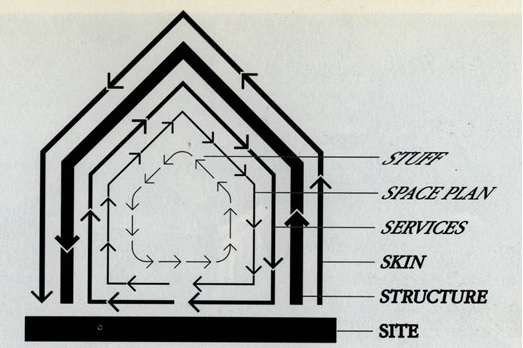
\includegraphics[width=3.5in]{figures/brand-diagram}
	\caption{The different layers of change \citep[chapter 2]{brand1995buildings}}
   \label{brand-diagram}
\end{figure}

The six S's describes the different layers of change, three describing the exterior: Site, Structure and Skin and three describing the interior: Services, Space plan and Stuff.
Each layer has a different rate of change, Site having the longest and Stuff the shortest rate of change, see figure~\ref{brand-diagram}.
As the rate of change differs for the different components of the building, the building is, as Brand notes, constantly `tearing itself apart', or in a more constructive term, constantly evolving.

Brand argues in favor for an approach where the inhabitants of a building can evolve and change the building over time according to their needs \citep{brandBBCvideo}.
He sees this in contrast to a scenario where a single person or group designs a building for others to use.
In light of this, providing inhabitants with higher rates of change could accommodate an even more dynamic relationship between the building and the people living in it.

We see two interesting ways of exploring this existing relationship between building and inhabitants.
One is to open up the layer of Stuff.
The layer of Stuff is all the things that gets moved around or changed on daily to monthly basis such as chairs and desks, kitchen appliances and lamps.
So what if Stuff could be changed, moved or modified on an even more frequent basis, say in minutes or hours, accommodating the need of the inhabitants with the possibility for them to adapt furniture and objects to current needs.

Another approach could be to pull down a given layer of change to a lower layer, for example enabling changes in the Space Plan as if it was Stuff, creating a more dynamic Space Plan.
This would open up for entirely new possibilities of rethinking the home. 
If, for example, homes had dynamic walls, ceilings, floors and doors that would give them a less static and permanent function, it could enable changes to the Space Plan that maybe lasts days or months, enabling the Space Plan to adapt to specific situations, just as you on the Stuff plan would add an extra chair to the table for a visiting guest. 

It is, of course, non trivial to make the home as dynamic and adaptable as suggested above.
But the this concept of the building as a living, ever-evolving entity, does give us inspiration to explore the use of digital systems in a domestic setting, as this could be one way to approach such a vision.
So with the help of computers and new materials we want to explore how we can accommodate and design for change in physical environment that surrounds us.
We want to explore how physical interfaces can be created on demand in an ad hoc manner, to better cope with the changes in the buildings space plan and on the level of stuff, and better accommodate the changing needs of its inhabitants.
As touched upon in chapter~\ref{ch:ui} this does somewhat challenge the traditional view of physical interfaces as they are generally considered static and permanent.
\todo{bedre afrunding til smart homes}
hvad skal der komme ud af det

Smart homes - ideen om det teknologiske hus
intro
definition/vision
complex setting
rodden - hvem skal deltage 

\section{Smart homes or home that make us smart}
\todo{section not done - needs work}

The idea of adding computer systems into the domestic environment is not a new one.
Ever since the emergence of electricity into the households, electrical appliances has been a part of the domestic setting.
And along with the increasingly more advanced appliances being developed, the dream and vision of even more sophisticated systems have continuously evolved

An early visual example of the fascination of `smart homes' is seen in the General Motors commercial film \emph{Design for Dreaming}\footnote{http://en.wikipedia.org/wiki/Design\_for\_Dreaming} from 1956 \citep{designfordreaming}, where the \emph{Home of the Future}\footnote{http://en.wikipedia.org/wiki/Home\_of\_the\_future} is presented.
Here we see a remote control of the different kitchen appliances, a (computer)screen that can show the final result of the recipe it is given, and a seemingly context-aware moving table.
Domestic technology appears even earlier where in the 1915-20, with the advent of electricity in common homes, electrically powered machines such as vacuum cleaners and refrigerators providing the `seedbed', as \citet{aldrich2003smart} puts it, for the emergence of the smart home.

In recent years, especially since Mark Weiser's vision of ubiquitous computing \citep{weiser1991computer}, a lot of the research in the domestic realm has focused on the idea of a \emph{home that is smart} where the goal is to use computers to make the home \emph{intelligent} \citep{taylor2007homes}.
\citet{aldrich2003smart} defines smart homes as:

\begin{quotation}
\emph{A ``smart home'' can be defined as a residence equipped with computing and information technology which anticipates and responds to the needs of the occupants, working to promote their comfort, convenience, security and entertainment through the management of technology within the home and connections to the world beyond.}
\end{quotation}
\citeauthor{aldrich2003smart} sees this definition as the acme of domestic technology as we can envision it today, putting it somewhere in between reality and fantasy.
\todo{mere her}

The domestic setting differs a lot from the traditional office setting where most research on ubiquitous computing has been conducted, and is in some ways even more complex as people in the domestic setting has a lot more freedom as to how they organize their space and time \cite{meyer2003survey}.
Also the aspect of user experience needs special consideration when introducing new technology to the home, whereas in a work setting the user might \emph{need} to use the new technology, imposed upon him by superiors, the technology for the home need to be usable and useful enough so that the user \emph{wants} to use \citep{meyer2003survey}.
\todo{maaske undlade naeste del}
A thorough look at the challenges related to creating ubiquitous computing for the home is presented by \citet{edwards2001home}.
Here Edwards et al. identifies seven challenges that need to be overcome before the vision of the ubiquitous smart home can become a reality. We will return to these challenges in relation to our own prototypes \todo{ref til prototype sektion}.

\citet{rodden2003evolution} have built upon Brands framework in the context of ubiquitous computing and the domestic setting and is therefore relevant for us here.
By looking at existing research Rodden et al. identifies three main approaches for creating interactive devices for domestic settings.

\begin{itemize}
  \item \emph{Information Appliance} that are stand-alone, self-contained devices that are often used as a layer of interactive functions on top of an existing appliance.
  \item \emph{Interactive Household Objects} that embeds interactive capabilities into existing household objects to create new means of interaction and communication, often building upon the existing understanding and metaphors associated with the household object.
  \item \emph{Augmented Furniture} that embeds sensory systems into furniture to add interactive capabilities. \ldots
\end{itemize}

Rodden et al. notes that the technology is most intrusive in information appliances, less so in interactive household objects and least in augmented furniture.

\todo{noget om bygninger ikke er nybyggerier og noget mere Rodden}
 
\todo{diskussion om empoverment, Brand/Rodden vs smart-homes/context-awareness/dubai-huse}

\todo{make systems that are not dictated by a designer, but made for adaptation and modification. People are different and have different, changing, needs. Systems needs to repsond to this}



Cite test:

\cite{abowd2012next} \cite{ishii1997tangible} \cite{ishii2012radical} \cite{weiser1991computer}


\chapter{Conclusion}
\label{ch:conclusion}
The apparent conclusion

\todo{\dots}

%%%%%%%%%%%%%%%%%%%%%%%%%%%%%%%%%%%%%%%%%%%%%%%%%%%%%%%%%%%%%%%%%%%%%%%

\addcontentsline{toc}{chapter}{Primary Bibliography}

\bibliographystyle{plainnat} 
\bibliography{refs}

%%%%%%%%%%%%%%%%%%%%%%%%%%%%%%%%%%%%%%%%%%%%%%%%%%%%%%%%%%%%%%%%%%%%%%%

\listoffigures
\listoftables

\end{document}

